\documentclass{article}
\usepackage[utf8]{inputenc}
\usepackage{amsmath}
\usepackage{amssymb}
\usepackage{geometry}
\usepackage{graphicx}
\usepackage{float}
\usepackage{tikz}
\usetikzlibrary{shapes.geometric, arrows, positioning, calc, patterns}

\geometry{a4paper, margin=1in}

\title{Model Extension: Author-Journal Game with Competition and Capacity Constraints}

\date{\today}

\begin{document}

\maketitle

\section{Motivation and Problem Statement}

In our previous evolutionary game-theoretic model of the author-journal interaction, we observed that the equilibrium strategies were largely insensitive to the population size $N$. This phenomenon arises because, in the original formulation, the payoff of a focal author depends solely on their own strategy and the journal's acceptance policy, but is independent of the actions of other authors. Consequently, there is no \textit{congestion effect} or \textit{competition} for limited resources.

To address this and model a more realistic academic publishing environment (e.g., conferences with fixed acceptance rates or journals with limited pages), we introduce a capacity threshold $K$. This mechanism creates a zero-sum element: as the number of submissions increases, the probability of acceptance for a passed paper decreases, potentially disincentivizing opportunistic strategies like \textit{Always Submit} (AS).

\section{The Threshold Competition Model}


The updated interaction proceeds in the following stages:
\begin{enumerate}
    \item \textbf{Submission:} $N$ authors choose a strategy $s \in \{OG, AS, \dots\}$.
    \item \textbf{Peer Review (Perception):} All submissions undergo peer review characterized by false negative rate $\epsilon$ and false positive rate $\lambda$. Papers that pass peer review enter a ``Perception Pool'' of size $M$.
    \item \textbf{Competition (Threshold Cut):} The journal has a maximum capacity $K$.
    \begin{itemize}
        \item If $M \le K$, all papers in the pool are accepted.
        \item If $M > K$, the journal randomly selects $K$ papers from the pool to accept. The remaining $M-K$ papers are rejected despite passing review.
    \end{itemize}
\end{enumerate}


Let $\alpha$ be the probability an author produces a good paper. The probability that a single author's submission passes the peer review stage, denoted as $P_{pass}(s)$, depends on their chosen strategy $s$:

\begin{align}
    P_{pass}(OG) &= \alpha(1-\epsilon) \\
    P_{pass}(AS) &= \alpha(1-\epsilon) + (1-\alpha)\lambda
\end{align}

Here, $OG$ authors only submit good papers, while $AS$ authors submit both good and bad papers, benefiting from the false positive rate $\lambda$.


\begin{figure}[htbp]
    \centering
    % 这一行让图片自动缩放适应页面宽度
    \resizebox{\textwidth}{!}{
        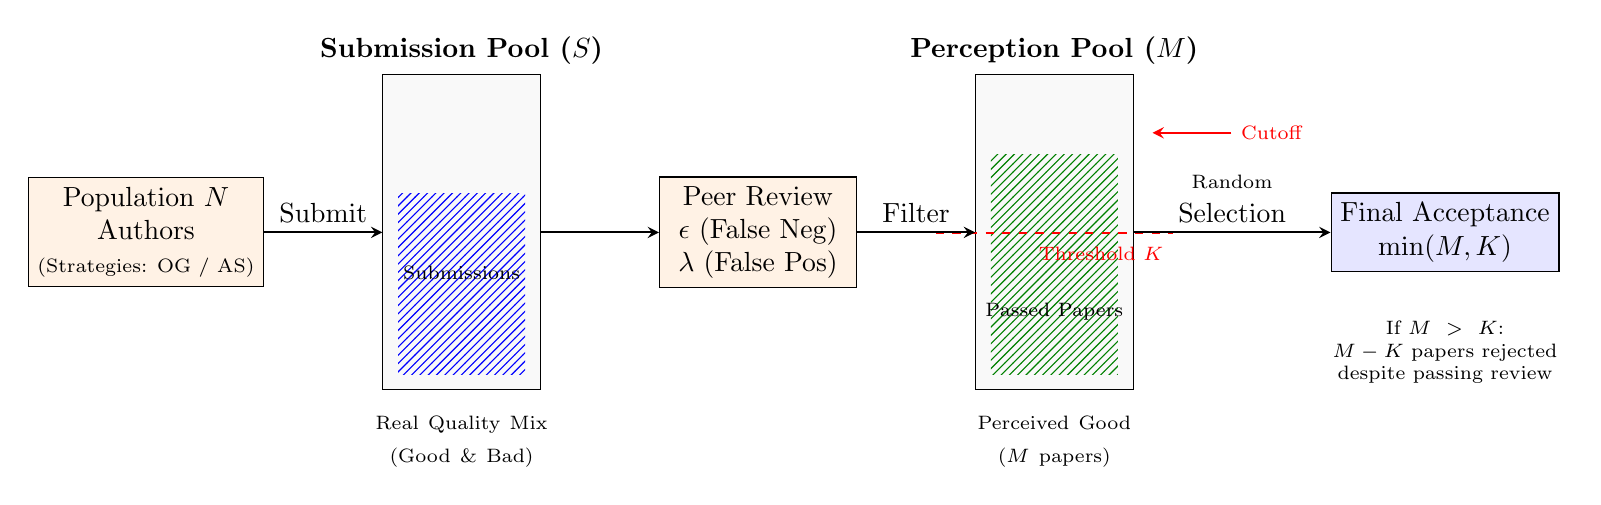
\begin{tikzpicture}[node distance=2cm, auto, >=stealth]

        % --- 定义样式 ---
        \tikzstyle{process} = [rectangle, minimum width=2.5cm, minimum height=1cm, text centered, draw=black, fill=orange!10]
        \tikzstyle{pool} = [rectangle, minimum width=2cm, minimum height=4cm, draw=black, fill=gray!5]
        \tikzstyle{arrow} = [thick,->]

        % --- 节点定义 ---

        % 1. Authors
        \node (authors) [process, align=center] {Population $N$ \\ Authors \\ \scriptsize (Strategies: OG / AS)};

        % 2. Submission Pool
        \node (submit_pool) [pool, right=1.5cm of authors, label=above:\textbf{Submission Pool ($S$)}] {};
        \fill[pattern=north east lines, pattern color=blue] ($(submit_pool.south west) + (0.2,0.2)$) rectangle ($(submit_pool.south east) + (-0.2, 2.5)$);
        \node at ($(submit_pool.south) + (0, 1.5)$) {\scriptsize Submissions};

        % 3. Peer Review
        \node (review) [process, right=1.5cm of submit_pool, align=center] {Peer Review \\ $\epsilon$ (False Neg) \\ $\lambda$ (False Pos)};

        % 4. Perception Pool
        \node (percep_pool) [pool, right=1.5cm of review, label=above:\textbf{Perception Pool ($M$)}] {};
        \fill[pattern=north east lines, pattern color=green!50!black] ($(percep_pool.south west) + (0.2,0.2)$) rectangle ($(percep_pool.south east) + (-0.2, 3.0)$);
        \node at ($(percep_pool.south) + (0, 1.0)$) {\scriptsize Passed Papers};

        % --- Threshold K (红色虚线与文字) ---
        \draw[red, thick, dashed] ($(percep_pool.south west) + (-0.5, 2.0)$) -- ($(percep_pool.south east) + (0.5, 2.0)$);
        % 文字在虚线右下方
        \node[text=red, anchor=north east, yshift=-0.05cm] at ($(percep_pool.south east) + (0.5, 2.0)$) {\scriptsize Threshold $K$};

        % 5. Final Selection
        \node (final) [process, right=2.5cm of percep_pool, align=center, fill=blue!10] {Final Acceptance \\ $\min(M, K)$};

        % --- 连线 ---
        \draw[arrow] (authors) -- node[above] {Submit} (submit_pool);
        \draw[arrow] (submit_pool) -- (review);
        \draw[arrow] (review) -- node[above] {Filter} (percep_pool);

        % --- Cutoff (Cutoff 在 Random Selection 上方,箭头向左) ---
        \draw[arrow] (percep_pool) -- node[above, align=center] (rand_sel) {\scriptsize Random\\Selection} (final);
        
        % Label
        \node[above=0.2cm of rand_sel, xshift=0.5cm, text=red] (cutoff_label) {\scriptsize Cutoff};
        % Arrow pointing LEFT
        \draw[->, red, thick] (cutoff_label.west) -- ++(-1.0, 0);

        % --- 底部注释 ---
        \node [below=0.2cm of submit_pool, text width=2.5cm, align=center] {\scriptsize Real Quality Mix\\(Good \& Bad)};
        \node [below=0.2cm of percep_pool, text width=2.5cm, align=center] {\scriptsize Perceived Good\\($M$ papers)};
        \node [below=0.5cm of final, text width=3cm, align=center, font=\scriptsize] {If $M > K$: \\ $M-K$ papers rejected \\ despite passing review};

        \end{tikzpicture}
    }
    \caption{\textbf{Schematic representation of the Threshold Competition Model.} The process unfolds in three stages: (1) Submission into a pool $S$; (2) Peer review filtering into a perception pool $M$; and (3) A hard capacity constraint $K$ (red dashed line). If $M > K$, a random cutoff occurs, rejecting surplus papers even if they passed review. This introduces the competition factor $\gamma$.}
    \label{fig:threshold_model}
\end{figure}
\section{Derivation of the Competition Factor $\gamma$}

The key addition to the payoff function is the competition factor $\gamma$, which represents the probability that a paper is finally accepted \textit{given that it has already passed peer review}.

Let us consider a \textit{focal author} who has passed peer review. Let $M_{-i}$ be the random variable representing the number of \textit{other} authors (out of $N-1$) whose papers also passed peer review.

The total number of passed papers is therefore $M = 1 + M_{-i}$.

The competition factor for the focal author is defined as:
\begin{equation}
    \gamma_{\text{focal}} = \min\left(1, \frac{K}{1 + M_{-i}}\right) = 
    \begin{cases} 
      1 & \text{if } 1 + M_{-i} \le K \\
      \frac{K}{1 + M_{-i}} & \text{if } 1 + M_{-i} > K
   \end{cases}
\end{equation}

\subsection{Expected Competition Factor}
Since $M_{-i}$ is a random variable, authors base their decisions on the expected value $E[\gamma_{\text{focal}}]$. 

Assume the population consists of $N_{OG}$ authors playing $OG$ and $N_{AS}$ authors playing $AS$ (where $N_{OG} + N_{AS} = N - 1$, excluding the focal author). The variable $M_{-i}$ is the sum of two independent binomial distributions:
\begin{equation}
    M_{-i} = X_{OG} + X_{AS}
\end{equation}
where $X_{OG} \sim B(N_{OG}, P_{pass}(OG))$ and $X_{AS} \sim B(N_{AS}, P_{pass}(AS))$.

The expected competition factor is given by:
\begin{equation}
    E[\gamma_{\text{focal}}] = \sum_{m=0}^{N-1} \Pr(M_{-i} = m) \cdot \min\left(1, \frac{K}{1 + m}\right)
\end{equation}


\section{Payoff after competition}





In this section, we rigorously define the payoff functions for both authors and journals under the Threshold Competition Model. The introduction of the capacity constraint $K$ and the endogenous competition factor $\gamma$ fundamentally alters the strategic landscape.

We first define the key variables used in the payoff derivation:

\begin{table}[h]
\centering
\begin{tabular}{cl}
\hline
\textbf{Symbol} & \textbf{Description} \\ \hline
$N$ & Total number of authors \\
$K$ & Journal capacity (maximum number of accepted papers) \\
$S$ & Total number of submissions (Submission Pool) \\
$M$ & Number of papers passing peer review (Perception Pool) \\
$\gamma$ & Competition factor, probability of acceptance after passing review \\
$\alpha$ & Probability that an author produces a good paper \\
$\epsilon$ & False negative rate (probability of rejecting a good paper) \\
$\lambda$ & False positive rate (probability of accepting a bad paper) \\
$r$ & Reward for an accepted paper (Author) \\
$c$ & Cost of submission (Author) \\
$B$ & Benefit for accepting a good paper (Journal) \\
$D$ & Penalty for accepting a bad paper (Journal) \\
$C(S)$ & Cost of reviewing $S$ submissions \\
\hline
\end{tabular}
\caption{Key notation and definitions.}
\label{tab:variables}
\end{table}

\subsection{Journal}

The journal's payoff is determined by the quality of the accepted papers minus the cost of reviewing. The crucial addition in this model is that the competition factor $\gamma$ is endogenous to the journal's strategy. The journal maximizes its utility by choosing a strategy $S_J \in \{OG, AA, OB, AR\}$.

The competition factor $\gamma$ is defined as the ratio of capacity $K$ to the size of the perception pool $M$, capped at 1:
\begin{equation}
    \gamma(S_J) = \min\left(1, \frac{K}{M(S_J)}\right)
\end{equation}
Since the screening policy (determined by effective $\epsilon$ and $\lambda$) changes the size of $M$, $\gamma$ varies across strategies. Let $S_{good}$ and $S_{bad}$ be the total number of good and bad papers submitted by the authors, such that $S = S_{good} + S_{bad}$.

\paragraph{Only Good (OG) -- Selective Strategy}
The journal applies standard peer review to filter papers, aiming to accept good papers and reject bad ones.
\begin{itemize}
    \item \textbf{Screening parameters:} Standard $\epsilon$ and $\lambda$.
    \item \textbf{Perception Pool ($M_{OG}$):} Contains accepted good papers and falsely accepted bad papers.
    \begin{equation}
        M_{OG} = S_{good}(1-\epsilon) + S_{bad}\lambda
    \end{equation}
    \item \textbf{Competition Factor ($\gamma_{OG}$):}
    \begin{equation}
        \gamma_{OG} = \min\left(1, \frac{K}{S_{good}(1-\epsilon) + S_{bad}\lambda}\right)
    \end{equation}
    \item \textbf{Payoff ($U_J(OG)$):} The journal gains $B$ from good papers and loses $D$ from bad papers, scaled by $\gamma_{OG}$.
    \begin{equation}
        U_J(OG) = \gamma_{OG} \left[ B \cdot S_{good}(1-\epsilon) - D \cdot S_{bad}\lambda \right] - C(S)
    \end{equation}
\end{itemize}

\paragraph{Always Accept (AA) -- Permissive Strategy}
The journal abandons screening, effectively setting $\epsilon=0$ and $\lambda=1$.
\begin{itemize}
    \item \textbf{Perception Pool ($M_{AA}$):} All submissions enter the pool.
    \begin{equation}
        M_{AA} = S = S_{good} + S_{bad}
    \end{equation}
    \item \textbf{Competition Factor ($\gamma_{AA}$):} This strategy maximizes congestion.
    \begin{equation}
        \gamma_{AA} = \min\left(1, \frac{K}{S}\right)
    \end{equation}
    \item \textbf{Payoff ($U_J(AA)$):}
    \begin{equation}
        U_J(AA) = \gamma_{AA} \left[ B \cdot S_{good} - D \cdot S_{bad} \right] - C(S)
    \end{equation}
\end{itemize}

\paragraph{Only Bad (OB) -- Irrational Strategy}
The journal adopts an inverse selection policy, accepting papers that are perceived as ``bad'' by the peer review process. This strategy effectively targets papers that fail the standard quality threshold.
\begin{itemize}
    \item \textbf{Perception Pool ($M_{OB}$):} The pool consists of good papers that were falsely rejected (false negatives) and bad papers that were correctly identified as bad (true negatives).
    \begin{equation}
        M_{OB} = S_{good}\epsilon + S_{bad}(1-\lambda)
    \end{equation}
    \item \textbf{Competition Factor ($\gamma_{OB}$):}
    \begin{equation}
        \gamma_{OB} = \min\left(1, \frac{K}{S_{good}\epsilon + S_{bad}(1-\lambda)}\right)
    \end{equation}
    \item \textbf{Payoff ($U_J(OB)$):} Although the journal intends to select bad papers, it may accidentally accept good papers due to review errors ($\epsilon$). However, it also accepts the vast majority of bad papers.
    \begin{equation}
        U_J(OB) = \gamma_{OB} \left[ B \cdot S_{good}\epsilon - D \cdot S_{bad}(1-\lambda) \right] - C(S)
    \end{equation}
    Note that despite the potential small gain from $B \cdot S_{good}\epsilon$, the term $-D \cdot S_{bad}(1-\lambda)$ typically dominates because $D > B$ and $(1-\lambda) \gg \epsilon$ in realistic settings. Thus, $U_J(OB)$ remains strictly dominated by strategies that do not actively seek penalties.
\end{itemize}

\paragraph{Always Reject (AR) -- Baseline Strategy}
The journal rejects all submissions. The perception pool is empty ($M=0$), and no papers are published.
\begin{itemize}
    \item \textbf{Payoff ($U_J(AR)$):}
    \begin{equation}
        U_J(AR) = 0
    \end{equation}
\end{itemize}

\subsection{Author}

An author chooses a strategy $S_A \in \{OG, OB, AS, NS\}$. The author's expected utility depends on the probability of producing a good paper ($\alpha$), the cost of submission ($c$), the reward ($r$), and the probability of acceptance. The probability of acceptance is a two-step process: passing the peer review (denoted as $P_{pass}$) and surviving the competition cut (denoted by $\gamma$).

The expected payoff is generally given by:
\begin{equation}
    U_A = P(\text{Good}) \cdot P(\text{Accept}|\text{Good}) \cdot r + P(\text{Bad}) \cdot P(\text{Accept}|\text{Bad}) \cdot r - \text{Total Cost}
\end{equation}

Assuming the journal plays the standard \textit{Only Good} strategy (implying the competition factor is $\gamma_{OG}$), the payoffs for the four author strategies are derived as follows:

\paragraph{Only Good (OG)}
The author submits only if the paper is good.
\begin{itemize}
    \item Probability of submission: $\alpha$
    \item Probability of passing review: $1-\epsilon$
    \item \textbf{Payoff:}
    \begin{equation}
        U_A(OG) = \alpha \left[ (1-\epsilon) \gamma_{OG} r - c \right]
    \end{equation}
\end{itemize}

\paragraph{Only Bad (OB)}
The author submits only if the paper is bad, attempting to exploit the false positive rate.
\begin{itemize}
    \item Probability of submission: $1-\alpha$
    \item Probability of passing review: $\lambda$
    \item \textbf{Payoff:}
    \begin{equation}
        U_A(OB) = (1-\alpha) \left[ \lambda \gamma_{OG} r - c \right]
    \end{equation}
\end{itemize}

\paragraph{Always Submit (AS)}
The author submits regardless of quality.
\begin{itemize}
    \item Probability of submission: $1$
    \item Probability of passing review: The paper passes if it is good and correctly identified ($1-\epsilon$), or if it is bad and falsely accepted ($\lambda$).
    \item \textbf{Payoff:}
    \begin{equation}
        U_A(AS) = \left[ \alpha(1-\epsilon) + (1-\alpha)\lambda \right] \gamma_{OG} r - c
    \end{equation}
\end{itemize}

\paragraph{Never Submit (NS)}
The author does not submit any papers.
\begin{itemize}
    \item \textbf{Payoff:}
    \begin{equation}
        U_A(NS) = 0
    \end{equation}
\end{itemize}




The assumption that these constraints hold is strictly necessary to model a functional and sustainable scientific community rather than a degenerate system. Specifically, the condition $c > \lambda r$ ensures that the ecosystem is not overwhelmed by costless speculative spamming; the lower bound on $\gamma$ posits that the journal has not reached a state of total collapse where even high-quality contributions are discouraged; and the reputation constraint on $D$ distinguishes legitimate, quality-seeking venues from predatory publishers. By restricting our analysis to this valid parameter space, we filter out trivial breakdown scenarios to focus exclusively on the non-trivial evolutionary dynamics: how resource scarcity ($K$) and congestion precipitate a tragedy of the commons, and how the interplay between institutional screening and authorial strategy can resolve it.

We incorporate $E[\gamma_{\text{focal}}]$ into the utility functions. Let $r$ be the reward for acceptance and $c$ be the cost of submission.


An $OG$ author submits with probability $\alpha$. If they submit, they pay cost $c$. They pass review with probability $1-\epsilon$. If they pass, they are accepted with probability $E[\gamma_{\text{focal}}]$.

\begin{equation}
    U_A(OG) = \alpha \left[ (1-\epsilon) \cdot E[\gamma_{\text{focal}}] \cdot r - c \right]
\end{equation}
\textit{Note: Assuming cost is paid per submission regardless of acceptance.}


An $AS$ author always submits (probability 1), paying cost $c$. They pass review with probability $P_{pass}(AS)$. If they pass, they are accepted with probability $E[\gamma_{\text{focal}}]$.

\begin{equation}
    U_A(AS) = \left[ (\alpha(1-\epsilon) + (1-\alpha)\lambda) \cdot E[\gamma_{\text{focal}}] \cdot r \right] - c
\end{equation}


The journal's utility depends on the quality of the final accepted papers and the cost of reviewing the total volume of submissions. 

Let $B$ be the benefit for accepting a good paper and $D$ be the penalty for accepting a bad paper.
The total submission volume $S$ is given by:
\begin{equation}
    E[S] = N_{OG} \cdot \alpha + N_{AS} \cdot 1
\end{equation}

The ``Perception Pool'' $M$ contains a mix of good and bad papers that passed review.
The expected number of good papers ($M_G$) and bad papers ($M_B$) in the pool are:
\begin{align}
    E[M_G] &= (N_{OG} + N_{AS}) \cdot \alpha(1-\epsilon) \\
    E[M_B] &= N_{AS} \cdot (1-\alpha)\lambda
\end{align}
\textit{Note: Both OG and AS authors contribute to $M_G$, but only AS authors contribute to $M_B$.}

Since the journal selects $K$ papers randomly from $M$ (if $M > K$), the final accepted papers maintain the same quality ratio as the pool. The expected acceptance rate for any paper in the pool is approximated by the system-wide competition factor $\bar{\gamma} = E[\min(1, K/M)]$.

The journal's expected payoff is:
\begin{equation}
    U_J = B \cdot (E[M_G] \cdot \bar{\gamma}) - D \cdot (E[M_B] \cdot \bar{\gamma}) - C(E[S])
\end{equation}

Where $C(S)$ is the cost function (e.g., linear or convex with respect to total submissions). This formulation highlights that while $K$ limits the absolute number of bad papers accepted (by reducing $\bar{\gamma}$), it does not improve the \textit{ratio} of good to bad papers, which is still determined by $\epsilon$ and $\lambda$.


\section{Conditional Dominated strategies}

To determine the evolutionary stability of the system, we perform a pairwise comparison of payoffs to identify strictly dominated strategies that can be eliminated from the strategy space. A strategy is considered strictly dominated if its expected utility is lower than that of another strategy under all admissible parameter configurations. Conversely, a strategy is conditionally viable if its dominance depends on specific inequalities involving the competition factor $\gamma$ and the penalty structure. 

We first analyze the author's strategy space. The strategy \textit{Never Submit} (NS) serves as the baseline with a fixed payoff of $U_A(NS) = 0$. Consider the \textit{Only Bad} (OB) strategy, where an author submits only bad papers to exploit the false positive rate $\lambda$. The expected payoff is $U_A(OB) = (1-\alpha)[\lambda \gamma r - c]$. Given the fundamental cost constraint $c > \lambda r$ (assuming submission costs exceed the expected reward of a lucky acceptance in a vacuum) and the fact that $\gamma \le 1$, the term $[\lambda \gamma r - c]$ is strictly negative. Consequently, $U_A(OB) < U_A(NS)$ holds universally, rendering OB a strictly dominated strategy. In contrast, the \textit{Only Good} (OG) and \textit{Always Submit} (AS) strategies are conditionally viable. $U_A(OG)$ remains positive as long as the competition factor satisfies $\gamma > c/[r(1-\epsilon)]$. Similarly, AS remains viable only when the dilution of acceptance probability $\gamma$ does not render the submission of bad papers prohibitively costly. Thus, the author's effective strategy space reduces to $\{OG, AS, NS\}$.

Next, we examine the journal's strategy space, using \textit{Always Reject} (AR) as the baseline with $U_J(AR)=0$. The \textit{Only Bad} (OB) strategy, representing an irrational inverse selection policy, yields a payoff of $U_J(OB) = \gamma_{OB} [ B S_{good}\epsilon - D S_{bad}(1-\lambda) ] - C(S)$. Although there is a non-zero probability $\epsilon$ of accepting a good paper by mistake, the operational parameters of a functional peer review system satisfy $(1-\lambda) \gg \epsilon$ and $D > B$. The penalty term from correctly identifying bad papers overwhelmingly dominates the accidental benefit term, ensuring $U_J(OB) < 0$ for any non-zero submission volume. Thus, Journal OB is strictly dominated by AR. The \textit{Always Accept} (AA) strategy is conditionally dominated. Its payoff $U_J(AA)$ becomes negative if the penalty for bad papers satisfies the reputation constraint $D > B (S_{good}/S_{bad})$. Under strict reputation mechanisms, AA is eliminated, leaving \textit{Only Good} (OG) as the sole dominant strategy for the journal, provided the screening costs do not exceed the utility of publishing good research. 

The complete classification of strategy dominance is summarized in Table \ref{tab:dominance_analysis}.

\begin{table}[!h]
\centering
\renewcommand{\arraystretch}{1.5}
\begin{tabular}{lp{5cm}lp{5cm}}
\hline
\textbf{Strategy} & \textbf{Payoff Function} & \textbf{Status} & \textbf{Condition / Reasoning} \\ \hline
\multicolumn{4}{l}{\textit{Author Strategies (Baseline: $U_A(NS)=0$)}} \\
Only Bad (OB) & $(1-\alpha)[\lambda \gamma r - c]$ & \textbf{Strictly Dominated} & Dominated by NS since $c > \lambda r$ and $\gamma \le 1$. \\
Only Good (OG) & $\alpha [(1-\epsilon)\gamma r - c]$ & Conditionally Viable & Viable if $\gamma > \frac{c}{r(1-\epsilon)}$. \\
Always Submit (AS) & $[\alpha(1-\epsilon) + (1-\alpha)\lambda]\gamma r - c$ & Conditionally Viable & Dominated by OG if congestion is high ($\gamma \to 0$); viable if $\gamma \to 1$ and costs are low. \\
Never Submit (NS) & $0$ & Survival & Optimal when competition is prohibitive. \\ \hline
\multicolumn{4}{l}{\textit{Journal Strategies (Baseline: $U_J(AR)=0$)}} \\
Only Bad (OB) & $\gamma_{OB}[B S_{good}\epsilon - D S_{bad}(1-\lambda)] - C(S)$ & \textbf{Strictly Dominated} & Dominated by AR. Penalties ($D$) outweigh accidental benefits ($B\epsilon$). \\
Always Accept (AA) & $\gamma_{AA}[B S_{good} - D S_{bad}] - C(S)$ & Conditionally Dominated & Dominated by AR if $D > B \frac{S_{good}}{S_{bad}}$. \\
Only Good (OG) & $\gamma_{OG}[B S_{good}(1-\epsilon) - D S_{bad}\lambda] - C(S)$ & \textbf{Dominant} & Strictly yields highest utility under standard parameters. \\
Always Reject (AR) & $0$ & Survival & Optimal only if system collapses ($U_J(OG) < 0$). \\ \hline
\end{tabular}
\caption{Pairwise comparison and dominance analysis of Author and Journal strategies under the Threshold Competition Model.}
\label{tab:dominance_analysis}
\end{table}
To establish the dynamic congestion model characterized by bistability (three equilibria), the game is governed by the following system of inequalities. Note that Condition (1) allows for conditional profitability of bad papers, which is essential for the survival of the "Always Submit" strategy.

\begin{equation}
\label{eq:dynamic_constraints}
\begin{cases}
    \textbf{(1) Profitability Condition:} & \lambda r > c \\
    \textbf{(2) Reputation Constraint:} & D > \frac{\alpha}{1-\alpha}B \\
    \textbf{(3) Viability Constraint:} & \gamma > \frac{c}{r(1-\epsilon)}
\end{cases}
\end{equation}

Where $c$ is the submission cost, $r$ is the reward for authors, $D$ is the damage to the journal, $B$ is the benefit to the journal, and $\lambda r$ represents the potential return of a bad paper if accepted.

\textbf{1. Elimination of Author Strategies}

The strategy \textbf{\{Never Submit\}}, defined as $\sigma_A = (NS|G, NS|B)$, is strictly dominated for Good ($G$) types due to the \textbf{Viability Constraint}.
\begin{align*}
    U_A(NS \mid G) &= 0 \\
    U_A(S \mid G) &= \gamma \cdot r \cdot (1-\epsilon) - c
\end{align*}
From inequality (3), we have $\gamma > \frac{c}{r(1-\epsilon)}$, implying $U_A(S \mid G) > 0$. Rational authors holding good papers will always submit.

The strategy \textbf{\{Only Bad\}}, defined as $\sigma_A = (NS|G, S|B)$, is eliminated due to the violation of \textbf{Monotonicity}, rather than cost.
While Inequality (1) $\lambda r > c$ implies that submitting a bad paper \textit{can} be profitable (if the Journal accepts), submitting a good paper is strictly \textit{more} profitable because the reward $r$ is strictly greater than the discounted reward $\lambda r$ (assuming $\lambda < 1$).
\begin{align*}
    U_A(S \mid G) &\approx r - c \\
    U_A(S \mid B) &\approx \lambda r - c
\end{align*}
Since $r > \lambda r$, we have $U_A(S \mid G) > U_A(S \mid B)$.
If a rational author chooses to submit a Bad paper ($S|B$), they must strictly prefer submitting a Good paper ($S|G$).
Therefore, the strategy $(NS|G, S|B)$ is strictly dominated by \textbf{\{Always Submit\}} $(S|G, S|B)$.

\textit{Note: Unlike the simplified static model, the strategy \textbf{\{Always Submit\}} is NOT dominated here, as Inequality (1) allows $U_A(S|B) > 0$ under conditions of high congestion (low screening).}

\textbf{2. Elimination of Journal Strategies}

The strategy \textbf{\{Always Accept\}}, defined as accepting all submissions, is eliminated due to the \textbf{Reputation Constraint}. The expected utility is:
\begin{align*}
    E[U_J(\text{Always Accept})] &= \alpha B - (1-\alpha) D
\end{align*}
From inequality (2), $(1-\alpha)D > \alpha B$, which implies $E[U_J] < 0$. The damage from bad papers outweighs the benefit of good ones in a blind acceptance scenario, forcing the journal to screen or reject.

The strategy \textbf{\{Only Bad\}}, defined as $\sigma_J = (R|G, A|B)$, is strictly dominated by rationality constraints:
\begin{align*}
    U_J(R \mid G) = 0 &< B = U_J(A \mid G) \\
    U_J(A \mid B) = -D &< 0 = U_J(R \mid B)
\end{align*}
This strategy minimizes utility in all states and is discarded.

The strategy \textbf{\{Reject All\}}, defined as $\sigma_J = (R|G, R|B)$, is dominated by the conditional strategy \{Only Good\}.
Since $U_J(A \mid G) = B > 0$, the Journal strictly prefers accepting Good papers over rejecting them. Thus, conditional acceptance dominates blanket rejection.

\textbf{Conclusion:}
The resulting reduced game consists of the strategies:
\begin{itemize}
    \item \textbf{Author:} $\mathcal{S}_A = \{\text{Only Good}, \text{Always Submit}\}$
    \item \textbf{Journal:} $\mathcal{S}_J = \{\text{Only Good}\}$
\end{itemize}
This strategy set allows for the evolutionary dynamics where the Author switches between "Only Good" and "Always Submit" based on the Journal's congestion-dependent screening effectiveness.



\section{Replicator Dynamics and Bifurcation Analysis}

\subsection{Reduction to a Two-Strategy System and Congestion Model}
Following the elimination of strictly dominated strategies (specifically \{Only Bad\} and \{Never Submit\}), the game is reduced to a dynamic contest between two Author strategies, while the Journal plays a fixed strategy of \textit{Only Good}. We define the population state $x \in [0, 1]$ as follows:
\begin{itemize}
    \item $x$: The proportion of Authors playing \textbf{\{Only Good\}}.
    \item $1-x$: The proportion of Authors playing \textbf{\{Always Submit\}}.
\end{itemize}

Since the Journal's strategy is fixed, the evolutionary dynamics are driven entirely by the payoff difference between the Author's two remaining strategies. To allow for the survival of the \textit{Always Submit} strategy and the emergence of complex dynamics, we assume the \textbf{Profitability Condition} ($\lambda B > c$) holds. This implies that submitting a "Bad" paper is profitable \textit{if} the journal fails to screen it.

\subsubsection{Physical Definitions and Variables}
We introduce a finite resource constraint on the Journal to model the \textbf{Congestion Effect}. The parameters are defined as follows:
\begin{itemize}
    \item $N$: Total population of authors.
    \item $K$: Journal processing capacity (total review effort available).
    \item $C_J$: Cost per review. Thus, $K/C_J$ represents the maximum number of papers the journal can effectively screen.
    \item $\alpha$: The prior probability that an author holds a "Good" paper.
    \item $B$: Benefit (Reward) of acceptance.
    \item $C$: Cost of submission.
    \item $D$: Reputational damage penalty for a rejected "Bad" paper.
    \item $\lambda$: The discount factor for a "Bad" paper (Payoff = $\lambda B$).
    \item $\epsilon$: A friction term to prevent singularities.
\end{itemize}

\subsection{Derivation of the Polynomial Dynamics}

To analyze the stability of the system, we express the rate of change $\frac{dx}{dt}$ as a function of the submission volume and screening effectiveness.

\subsubsection{Volume and Screening Functions}
The total submission volume $V(x)$ depends on the strategy distribution. "Only Good" authors submit with probability $\alpha$, while "Always Submit" authors submit with probability 1:
\begin{equation}
    V(x) = N [ \alpha x + (1 - x) ] = N [ 1 - (1 - \alpha)x ]
\end{equation}
Note that $V(x)$ is linear and decreasing in $x$; as honesty increases, junk submissions decrease.

The screening probability $\sigma(x)$ is endogenous and depends on the ratio of capacity to volume:
\begin{equation}
    \sigma(x) = \frac{K}{C_J \cdot V(x) + \epsilon}
\end{equation}
This inverse relationship creates the nonlinearity required for bistability.

\subsubsection{Utility Functions and Replicator Equation}
The evolutionary dynamics depend on the expected utility of submitting a "Bad" paper, $E[U_{Bad}]$.
\begin{itemize}
    \item If screened (probability $\sigma$): Payoff is $-C - D$.
    \item If unscreened (probability $1-\sigma$): Payoff is $\lambda B - C$.
\end{itemize}
The expected utility is:
\begin{align}
    E[U_{Bad}](x) &= \sigma(x) (-C - D) + (1 - \sigma(x)) (\lambda B - C) \nonumber \\
    &= \sigma(x) (-D - \lambda B) + (\lambda B - C)
\end{align}

Substituting this into the standard replicator equation $\frac{dx}{dt} = -x(1-x)(1-\alpha)E[U_{Bad}]$, and clearing the denominator $(C_J V(x) + \epsilon)$, we derive the polynomial $P(x)$ that characterizes the sign of the dynamics:
\begin{equation}
    P(x) = \underbrace{x(1-x)}_{\text{Deg 2}} \cdot \underbrace{\Big[ K(-D - \lambda B) + (\lambda B - C)(C_J N(1 - (1-\alpha)x) + \epsilon) \Big]}_{\text{Deg 1}}
\end{equation}

\subsubsection{Degree Analysis and Root Configuration}
The polynomial $P(x)$ is of \textbf{Degree 3 (Cubic)}. This is confirmed by the product of the quadratic replicator term $x(1-x)$ and the linear volume term nested within the utility function. Consequently, the system admits up to three real roots in $[0, 1]$:
\begin{enumerate}
    \item $x=0$: \textbf{Full Corruption} (Stable if congestion makes cheating profitable).
    \item $x=1$: \textbf{Ideal Honesty} (Stable if low volume makes screening strict).
    \item $x=x^*$: An internal \textbf{Tipping Point} (Unstable).
\end{enumerate}

The analytical form of the internal root is derived as:
\begin{equation}
    x^* = \frac{1}{1-\alpha} \left[ 1 + \frac{\epsilon}{C_J N} - \frac{K (D + \lambda B)}{C_J N (\lambda B - C)} \right]
\end{equation}

\subsection{Numerical Simulation and Parameter Analysis}

\subsubsection{Case 1: The Failure of Congestion ($K=500$)}
In the initial simulation with $N=1000$ and $K=500$, the journal capacity was sufficient to screen all papers even at maximum volume ($N$). Mathematically, this resulted in $x^* < 0$. Under these conditions, the effective screening rate $\sigma \approx 1$ rendered cheating globally unprofitable ($U_{Bad} < 0$), collapsing the game to a single stable equilibrium at $x=1$.

\subsubsection{Case 2: The Emergence of Bistability ($K=100$)}
By reducing capacity to $K=100$, we induced the congestion effect. At $x=0$, high volume overwhelms the journal ($\sigma$ is low), satisfying the profitability condition $\lambda B > C$. At $x=1$, volume is low, $\sigma$ is high, and cheating is punished. This trade-off creates the internal root $x^*$.

\begin{figure}[hbt!]
    \centering
    \includegraphics[width=0.9\textwidth]{polynomial_graph_1.png}
    \caption{Replicator Dynamics $\frac{dx}{dt}$ vs $x$ with $K=100$. The system exhibits bistability. The internal root $x^* \approx 0.786$ acts as an unstable repeller. If the initial proportion of honest authors $x < x^*$, the system collapses to full corruption ($x=0$). If $x > x^*$, it converges to full honesty ($x=1$).}
    \label{fig:replicator_dynamics}
\end{figure}

Figure \ref{fig:replicator_dynamics} visualizes this dynamic. The existence of $x^*$ in $(0, 1)$ confirms that the "Always Submit" strategy is viable only when the journal is congested.

\subsubsection{Impact of Population ($N$) and Capacity ($K$)}
We performed a parameter sweep to analyze how the tipping point $x^*$ shifts with $N$ and $K$.

\begin{figure}[hbt!]
    \centering
    \includegraphics[width=0.9\textwidth]{impact_N_K.png}
    \caption{Heatmap of the internal equilibrium $x^*$ relative to Total Authors ($N$) and Journal Capacity ($K$). The color gradient represents the position of the tipping point.}
    \label{fig:heatmap_nk}
\end{figure}

\textbf{Analysis of Figure \ref{fig:heatmap_nk}:}
\begin{itemize}
    \item \textbf{White Region (Right):} Represents parameters where $K$ is high relative to $N$. Here, the inequality $c > \lambda B$ effectively holds due to strict screening. No internal root exists, and honesty ($x=1$) is the only equilibrium.
    \item \textbf{Colored Region (Left):} Represents the "Congestion Zone" where $\lambda B > c$ is activated by low screening rates. As $N$ increases (moving up), the region of corruption expands (darker colors), indicating that a larger critical mass of honest authors is required to stabilize the system.
\end{itemize}

\end{document}



